\section{Zielplattform, Sensorik und Aktorik}
In diesem Projekt wird ein \ac{BBB} in Kombination mit einer Linux-Distribution verwendet um die digitale Regelung zu realisieren. Die Plattform basiert auf einem AM335x Sitara ARM Cortex-A8 Prozessor, der mit einer Taktrate von 1GHz betrieben wird. Des weiteren steht eine single precision NEON FPU, für die Berechnung von Gleitkommaoperationen, zur Verfügung. Diese Rechnerarchitektur reduziert die nötige Rechenezit für gewöhnliche Filter- und Regelungsalgorithmen auf wenige Mikrosekunden. Somit kann die, durch die Rechnung resultierende Totzeit, des digitalen Systems bei dem Reglerentwurf vernachlässigt werden.
Das Linux-Betriebssystem bringt weitere Vorteile für die Entwicklung des Gesamtsymtems mit sich. Zunächst existiert eine Vielzahl von Werkzeugen für die Entwicklung von Embbeded-Linux-Anwendungen. Dadurch wird der nötige Zeitaufwand für die Implementierung des Reglerprogramms reduziert werden. Des weiteren kann bei der Entwicklung auf Pakete und Bibliotheken der Linux-Gemeinde zurückgegriffen werden. Somit können auch komplexe Subsysteme, wie z.B. der hier verwendete TCP/IP-Server, in das Gesamtsystem eigebettet werden. Zuletzt kann das Dateisystem genutzt werden um Konfigurationen für Filter- und Regleralgorithmen auszutauschen, wodurch die Erprobung von verschiedenen Reglerkonzepten vereinfacht wird. 
Allerdings muss der Einfluss des Betriebssystem auf das Zeitverhalten der Regelung kritisch betrachtet werden. Einerseits kann die Abtastung an äquidistanten Stützstellen nicht mehr garantiert werden. Anderseits entsteht durch die Verwendung von Linux-Treibern Verzögerungen, die zu weiteren Totzeiten führen.

Deshalb wird zunächst die verwendete Peripherie und deren softwareseite Auswertung vorgestellt. Auf dem Würfelgehäuse sind insgesamt sechs MPU9250-Module[Datenblatt MPU] montiert. Die Module besitzen jeweils einen Beschleunigungs- und Drehratensensor, welche genutzt werden um einen Teil des Zustandvektors zu bestimmen. Die Kommunikation zwischen den Sensormodulen und dem \ac{BBB} erfolgt über einen \ac{SPI}-Bus. Das das \ac{SPI}-Modul des \ac{BBB} nur einen \ac{CS}Pin besitzt wird dieser über einen AnalogSwitch[DatenBlatt] mit den Sensoren verbunden.
\begin{figure}[!h]
\centering
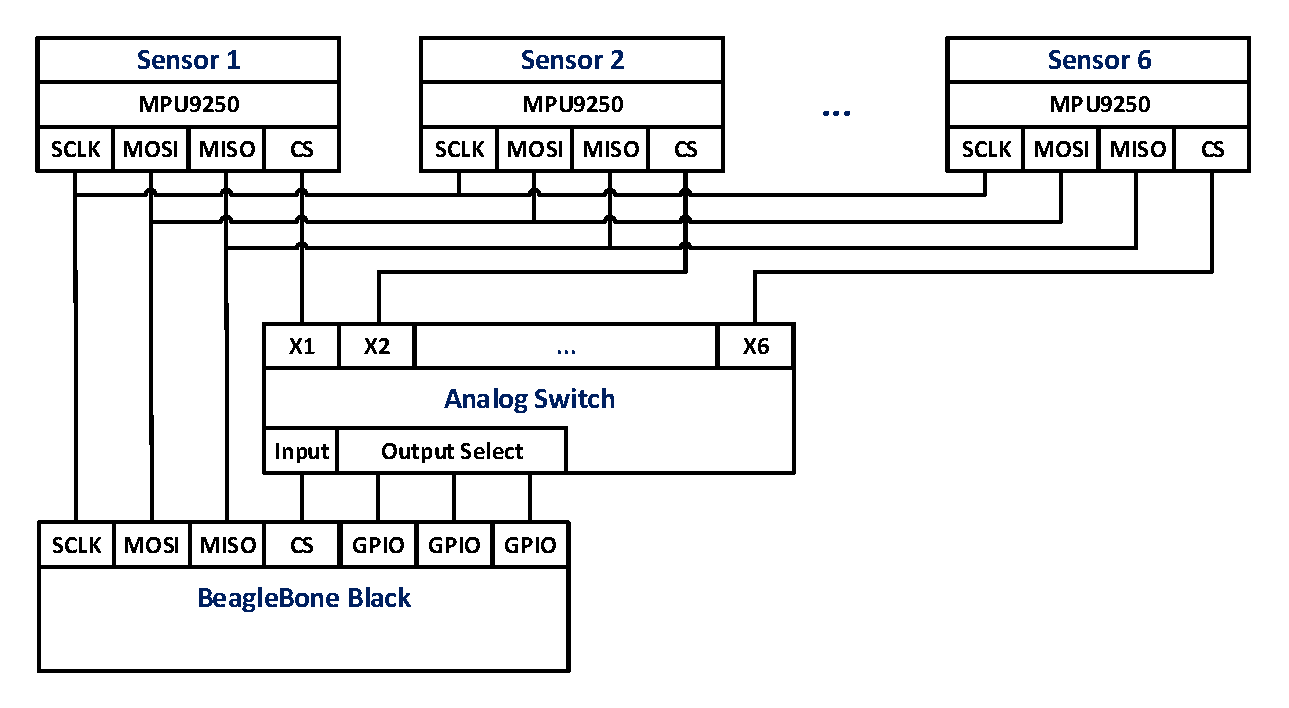
\includegraphics[width=0.7\linewidth]{img/SW_0_Sensoren_BSB.pdf}
\caption{Blockschaltbild Sensorkommunikation}
\end{figure}
Drei digitale Ausgänge des \ac{BBB} sind mit den Steuereingängen des Schalters verbunden um die \ac{CS}-Leitung auf den Ausgang des gewünschten Sensors zu legen.
Im Quellcode werden die Peripheriegeräte durch Klassen repräsentiert. Für die Steuerung der Digitalausgänge wird die Klasse \textit{CGPIO} implementiert, welche als Konstruktorargument die Nummer des zu konfigurierenden Pins entgegennimmt. Des weiteren betet sie Methoden zum Setzen bzw. Rücksetzen des Ausgangs. Hierfür wird die Schnittstelle des Treibers im Dateisystem verwendet. Zur Steuerung des Switches wird die Klasse \textit{CSwitch} aus drei Instanzen des Typs \textit{CGPIO} komponiert und implementiert die Methoden \textit{selectXi()} um die Schalterausgänge auszuwählen.
Analog wird für die Konfiguration und Auswertung der Sensoren die Klasse \textit{CMPU9250} implementiert. Zur Interaktion mit dem \ac{SPI}-Treiber wird die Posix-Funktion \textit{ioctl()} verwendet, welche zu einer kürzeren Ausführungszeit der Treiberaufrufe führt und im Vergleich zu der Dateisystemschnittstelle detaillierte Konfigurationsoptionnen bietet. Die Klasse nutzt die \ac{SPI}-Schnittstelle um die Sensoren in der \textit{init()}-Methode zu konfigurieren. Anschießend können über die Methode \textit{fetchData()} die aktuellen Beschleunigungs- und Winkelgeschwindigkeitswerte ausgelesen werden.

Die letztendliche Anwenderschnittstelle bietet die Klasse \textit{CSensorSystem}, welche aus einer Instanz des Typ \textit{CSwitch} und \textit{CMPU9250} komponiert wird. Im Konstruktur werden die sechs Sensoren initialisiert und anschließend über die Methode \textit{fetchSensorData()} ausgelesen. Die Daten werden in der Struktur \textit{SSensorData} gespeichert, welche Membervariablen für die Messwerte besitzt.
\begin{figure}[!h]
\centering
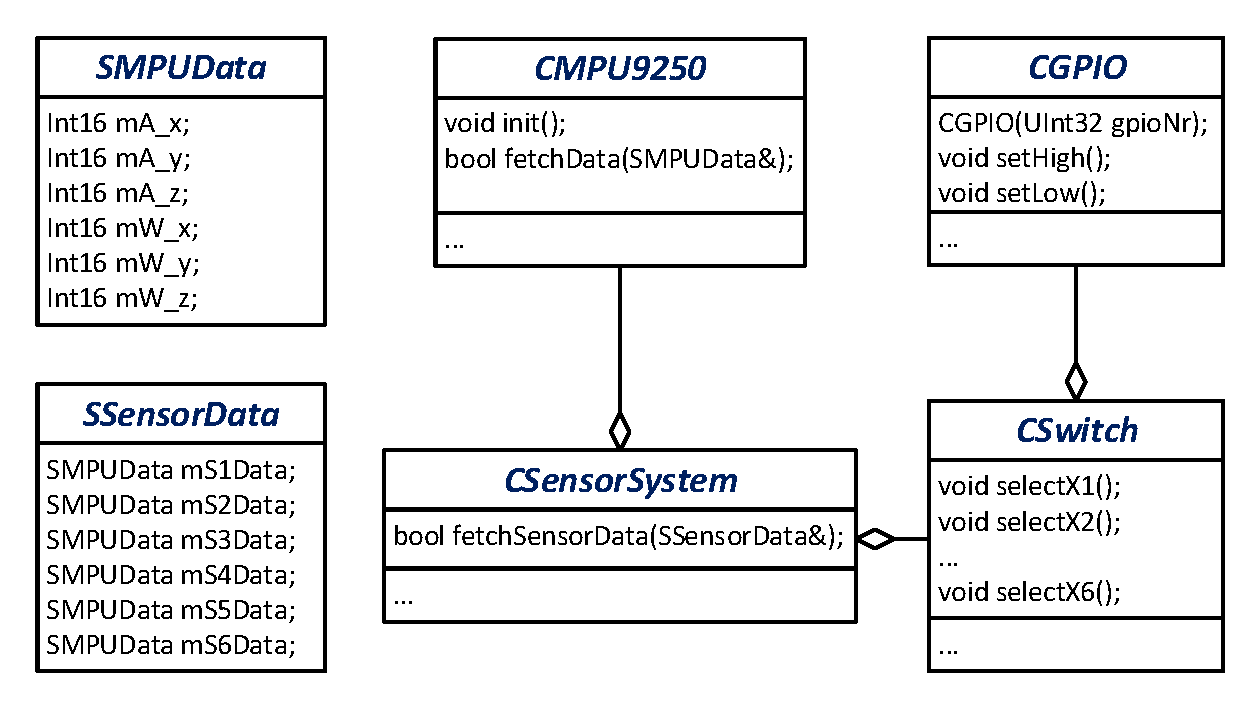
\includegraphics[width=0.7\linewidth]{img/SW_0_Sensoren_KD.pdf}
\caption{Klassendiagramm der Sensorschnittstelle}
\end{figure}

Die Stellgrößen der Regelung werden durch drei Motoren generiert, die jeweils über einen Treiberbaustein kontrolliert werden. Jeder Motortreiber ist mit zwei digitalen Ausgängen verbunden. Diese steuern die Freigabe und Drehrichtung des Motors. Die Vorgabe des Drehmoments erfolgt über ein \ac{PWM}-Signal. Zusätzlich erfassen die Motortreiber die Drehzahl und geben diese in Form eines Analogsignals an das \ac{BBB} zurück.
\begin{figure}[!h]
\centering
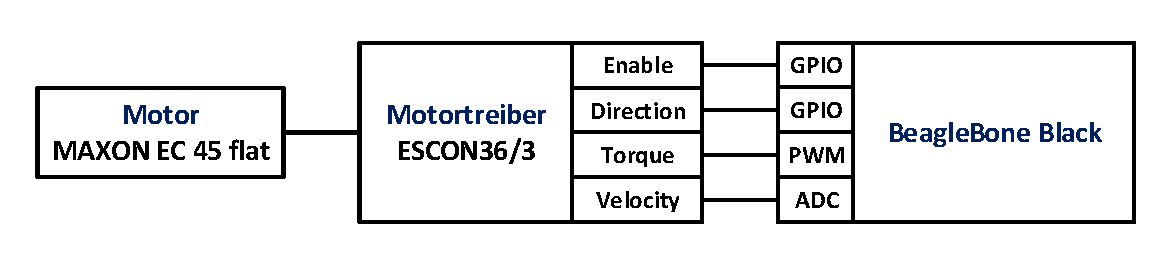
\includegraphics[width=0.7\linewidth]{img/SW_0_Motoren_BSB.pdf}
\caption{Blockschaltbild der Motoransteuerung} 
\end{figure}
Die Klasse \textit{CPWM} ermöglicht das Setzen eines Duty-Cycles, wobei die Treiberschnittstelle im Dateisystem verwendet wird. Eine Instanz dieser Klasse wird in \textit{CMotor} genutzt um das gewünschte Drehmoment einzustellen. Des weiteren werden zwei Instanz von \textit{CGPIO} genutzt um die Freigabe und Drehrichtung des Motors einzustellen. Für das Auslesen der \ac{ADC}-Werte wird ebenfalls eine Klasse \textit{C\ac{ADC}} angelegt. Da der Linux-Treiber für die Nutzung der AD-Wandler teilweise fehlerhaft ist wird ein alternative Vorgehensweise zur Nutzung der Peripherie genutzt. Hierbei wird mittels der Posix-Funktion \textit{mmap()} der Adressbereich der \ac{ADC}-Peripherie in den Userspace gelegt. Dadurch kann in der Anwendung direkt auf die \ac{ADC}-Register zugegriffen werden. Durch diesen Ansatz ergeben sich zwei Vorteile. Einerseits werden dem Nutzer keine Einschränkungen durch die Treiberschnittstelle aufgezwungen. Andererseits wird die nötige Zeit der AD-Wandlung durch den direkten Zugriff auf die Register reduziert. Allerdings ist diese Vorgehensweise mit einem größeren Implementierungsaufwand verbunden und wird deshalb nur genutzt wenn die Einschränkungen des Treibers nicht annehmbar sind.
die Klasse \textit{CSensorSystem} wird um eine Instanz von \textit{CADC} erweitert und umfasst somit die vollständige Sensorik des Systems. Um die Peripherie vollständig zu kapseln wird die Klasse \textit{CHardware} aus einer Instanz von \textit{CMotor} und \textit{CSensorSystem} komponiert.
\begin{figure}[!h]
\centering
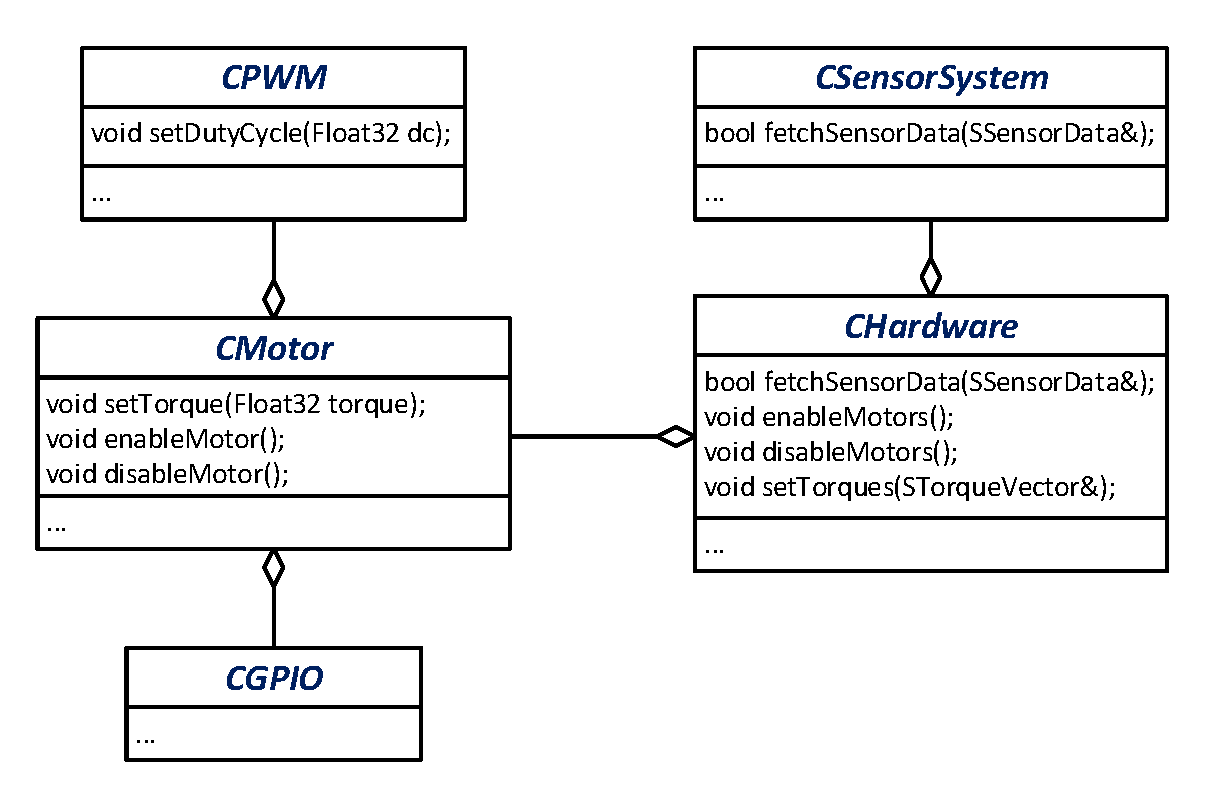
\includegraphics[width=0.7\linewidth]{img/SW_0_Hardware_KD.pdf}
\caption{Klassendiagramm der Hardwareansteuerung}
\end{figure}